\section{Results}
\label{sec:results}

\begin{table}[t]
  \caption{Warmup matters and attention scaling does not. Mean over \valSeeds{} seeds, with the range from the
  lowest to the highest seed in brackets; the best mean in each column is in bold.
  \emph{Capped}: no ramp, learning rate capped at the warmup peak (follow-up control).}
  \label{tab:results}
  \centering
  \small
  % Generated by figures_scripts/results_table.py. Do not edit by hand.
\begin{tabular}{lccccc}
\toprule
Configuration & Warmup & Scaling & Accuracy (\%) & Alignment (\%) & Final loss \\
\midrule
Baseline & yes & yes & 99.8 {\scriptsize [99.4, 100.0]} & \textbf{100.0} {\scriptsize [100.0, 100.0]} & \textbf{0.53} {\scriptsize [0.53, 0.53]} \\
No scaling & yes & no & \textbf{100.0} {\scriptsize [100.0, 100.0]} & \textbf{100.0} {\scriptsize [100.0, 100.0]} & \textbf{0.53} {\scriptsize [0.53, 0.53]} \\
No warmup & no & yes & 0.0 {\scriptsize [0.0, 0.0]} & 13.2 {\scriptsize [12.7, 13.6]} & 2.33 {\scriptsize [2.27, 2.36]} \\
Neither & no & no & 0.0 {\scriptsize [0.0, 0.0]} & 12.8 {\scriptsize [12.5, 13.2]} & 2.28 {\scriptsize [2.26, 2.31]} \\
No ramp, capped & capped & yes & 32.9 {\scriptsize [0.0, 98.6]} & 44.1 {\scriptsize [17.1, 95.3]} & 1.51 {\scriptsize [0.55, 2.07]} \\
\bottomrule
\end{tabular}

\end{table}

\begin{figure}[t]
  \centering
  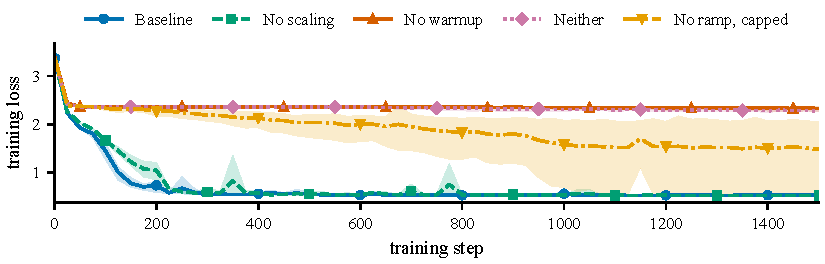
\includegraphics[width=\linewidth]{figures/loss_curves.pdf}
  \caption{Without warmup, training stalls almost immediately. Training loss for the four
configurations and the follow-up control (mean over
  \valSeeds{} seeds; shaded: range over seeds). With warmup, the two mean curves nearly coincide after
  early training; the shaded bands show brief loss spikes in single seeds. The capped no-ramp control improves slowly and solves the task in
  \valRampSolved{} of \valRampRuns{} seeds.}
  \label{fig:loss}
\end{figure}

\paragraph{Warmup matters.} The four configurations of Table~\ref{tab:results} split cleanly by warmup. With
warmup, every run solves the task: the baseline reaches \valAccBaseline\% exact-match accuracy (range
\valAccMinBaseline--\valAccMaxBaseline\%). Without warmup, all \valRunsNoWarmup{} runs fail, with accuracy of
\valAccNoWarmup\% with scaling and \valAccNoWarmupNoScaling\% without it. Their loss stops improving by step \valStallStep{} and stays between \valStallLow{} and \valStallHigh{} for the
rest of training, while the runs with warmup reach a final loss of \valLossBaseline.

\paragraph{The ramp itself matters, not only the initial learning rate.} Without warmup the learning rate starts at
$\valStartLRNoWarmup$, far above the warmup peak, so the failures above could come from the large learning rate rather
than from the missing ramp. The follow-up control removes the ramp but never exceeds the warmup peak. It solves the
task (accuracy of at least \valSolveThreshold\%) in \valRampSolved{} of \valRampRuns{} seeds, with mean accuracy
\valAccNoRampCapped\% (range \valAccMinNoRampCapped--\valAccMaxNoRampCapped\%); in the other \valRampUnsolved{} seeds the
loss falls only slowly and ends far above that of the baseline (Figure~\ref{fig:loss}). The ramp therefore matters at this learning
rate, but it is not strictly necessary for every seed. A rerun of the baseline with the control's code reproduced the
original baseline (largest difference in accuracy or final loss: \valRerunMaxDiff).

\paragraph{Attention scaling does not change the outcome here.} With warmup, removing the scaling gives
\valAccNoScaling\% accuracy and a final loss of \valLossNoScaling{} (baseline: \valLossBaseline), and the loss
curves differ only early in training and in brief loss spikes of single seeds (Figure~\ref{fig:loss}). Without warmup, keeping the scaling does not rescue training either.

\paragraph{The successful runs learn the expected alignment.} In both configurations with warmup, an
encoder--decoder attention head attends to the source token being copied at \valAlignBaseline\% (baseline) and
\valAlignNoScaling\% (no scaling) of target positions. For the failed runs it is \valAlignNoWarmup\%, close to the \valChanceAlign\% expected if the
strongest attention fell on a random source position.
